\chapter{Question3}
\section{问题概述}
%
%%对问题的直观描述
%
本问题要求实现Alpha-Beta剪枝算法,其中正方只有一个智能体,即吃豆人,但是反方,即幽灵,可能有多个。
%
%对项目已有代码的阅读和理解
%
%
%解决问题的思路和想法
%
\section{算法设计}
%
%用自己的语言描述解决问题所使用的算法的原理及功能,设计思路和算法流程图
%
题目中明确要求不能对子节点进行重排序,同时不修剪掉和得分和已有Alpha,Beta值相同的子树。

\begin{algorithm}[h]
    \SetKw{maximize}{maximize} 
    dummy,action = \maximize(gameState,1,$-\infty$,$\infty$)\tcp*[h]{这里无需返回的分数}\;
    \Return{action}
    \caption{Alpha-Beta(gameState)}
\end{algorithm}

\begin{procedure}[h]
    \KwOut{bestScore,bestAction}
    \SetKw{in}{in}
    \SetKw{minimize}{minimize}
    \tcp*[h]{给定状态和对应深度,返回从当前状态出发所能达到的最佳分数和对应的动作}\;
    actions = gameState.getLegalActions()\;
    ghostNum = gameState.getNumAgent - 1\;
    \If{depth > depthLimit or actions == None}
    {\Return{evaluationFunction(gameState),None}\tcp*[h]{无法继续行动,直接返回当前状态的分数}}
    bestScore = $-\infty$\;
    bestAction = None\;
    \ForEach{action \in actions}
    {
        next = gameState.generateSuccessor(gameState,action)\tcp*[h]{获取下一个状态}\;
        score,dummy = \minimize(next,1,ghostNum,depth,alpha,beta)\tcp*[h]{这里并不需要返回的动作}\;
        \If{score > bestScore}
        {
            bestAction = action\;
            bestScore = score\;
        }
        \lIf(\tcp*[h]{被剪枝}){score>beta}{\Return{bestScore,bestAction}}
        \lIf(\tcp*[h]{更新alpha值}){bestScore>alpha}{alpha = bestScore}
    }
    \Return{bestScore,bestAction}
    \caption{maximize(gameState,depth,alpha,beta)}
\end{procedure}

\begin{procedure}[h]
    \KwOut{bestScore,bestAction}
    \SetKw{in}{in}
    \SetKw{minimize}{minimize}
    \tcp*[h]{给定状态和对应深度,返回从当前状态出发所能达到的最佳分数和对应的动作}\;
    actions = gameState.getLegalActions()\;
    \If{depth > depthLimit or actions == None}
    {\Return{evaluationFunction(gameState),None}\tcp*[h]{无法继续行动,直接返回当前状态的分数}}
    bestScore = $\infty$\;
    bestAction = None\;
    \ForEach{action \in actions}
    {
        next = gameState.generateSuccessor(gameState,action)\tcp*[h]{获取下一个状态}\;
        \eIf{ghostNo == ghostNum}
        {
            score,dummy = \maximize(next,depth+1,alpha,beta)\tcp*[h]{当前智能体是最后一个幽灵,下一层为吃豆人}
        }
        {
        score,dummy = \minimize(next,ghostNo,ghostNum,depth,alpha,beta)\tcp*[h]{这里并不需要返回的动作}
        }
        \If(\tcp*[h]{对于幽灵而言,目标是让吃豆人的分数尽可能的低}){score < bestScore}
        {
            bestAction = action\;
            bestScore = score\;
        }
        \lIf(\tcp*[h]{被剪枝}){score<alpha}{\Return{bestScore,bestAction}}
        \lIf(\tcp*[h]{更新beta值}){bestScore<beta}{beta = bestScore}
    }
    \Return{bestScore,bestAction}
    \caption{minimize(gameState,ghostNo,ghostNum,depth,alpha,beta)}
\end{procedure}
Alpha-Beta剪枝算法只是在Minimax的算法基础上略作改动,但是却能够在性能上得到很大提升。其核心思想在于维护两个值:Alpha和Beta,分别记录
从博弈树根节点到当前结点的路径上的正方和反方的最佳选择。在Minimax算法中,虽然算法最终给出的只是从根节点出发的下一步,但是它的背后是博弈树上的一整条从
根节点到某一叶子结点的路径,因此,如果我们可以证明某一结点不会处于该路径上,那么以这一结点为根节点的子树便可以被剪枝掉了。

对于正方的结点,如果它的子节点上的值大于Beta值,那么它自身也肯定大于Beta。由于对于反方而言,Beta值对应着另外一条不经过该结点的更优的解,所以
最终反方选取的最优解肯定不会包含该节点,从而我们可以将该结点及其子树剪枝掉。对于反方的结点亦然。
\section{算法实现}
\begin{lstlisting}[emph={[3]currentGameState,gameState,depth,alpha,beta,ghostNo,ghostNum},emphstyle={[3]\color{vscode_parametercolor}},emph={[4]GameState,MinimaxAgent,AlphaBetaAgent},emphstyle={[4]\color{vscode_classcolor}}]
class AlphaBetaAgent(MultiAgentSearchAgent):
    def maximize(self, gameState: GameState, depth: int, alpha: float, beta: float):
        actions = gameState.getLegalActions(0)
        if depth > self.depth or not actions:
            return self.evaluationFunction(gameState), None
        bestScore = -float('inf')
        bestAction = None
        for action in actions:
            next = gameState.generateSuccessor(0, action)
            score, _ = self.minimize(next, 1, gameState.getNumAgents() - 1, depth, alpha, beta)
            if score > bestScore:
                bestAction = action
                bestScore = score
            if score > beta:
                return bestScore, bestAction
            if bestScore > alpha:
                alpha = bestScore
        return bestScore, bestAction

    def minimize(self, gameState: GameState, ghostNo: int, ghostNum: int, depth: int, alpha: float, beta: float):
        actions = gameState.getLegalActions(ghostNo)
        if not actions:
            return self.evaluationFunction(gameState), None
        bestScore = float('inf')
        bestAction = None
        for action in actions:
            next = gameState.generateSuccessor(ghostNo, action)
            if ghostNo == ghostNum:
                score, _ = self.maximize(next, depth + 1, alpha, beta)
            else:
                score, _ = self.minimize(next, ghostNo + 1, ghostNum, depth, alpha, beta)
            if score < bestScore:
                bestScore = score
                bestAction = action
            if score < alpha:
                return bestScore, bestAction
            if bestScore < beta:
                beta = bestScore
        return bestScore, bestAction

    def getAction(self, gameState: GameState):
        return self.maximize(gameState, 1, -float('inf'), float('inf'))[1]
\end{lstlisting}
\section{实验结果}
%
%对试验结果进行详细展示,对每个问题展示测试截图,对于测试用例进行描述说明,对于为通过测试的用例结合自己的算法进行分析,可以结合调试过程进行分析
%
我成功获得了本问题的所有分数,图\ref{q3}为实验结果。测试用例与问题2中所使用的一致。
\begin{figure}[H]
    \centering
    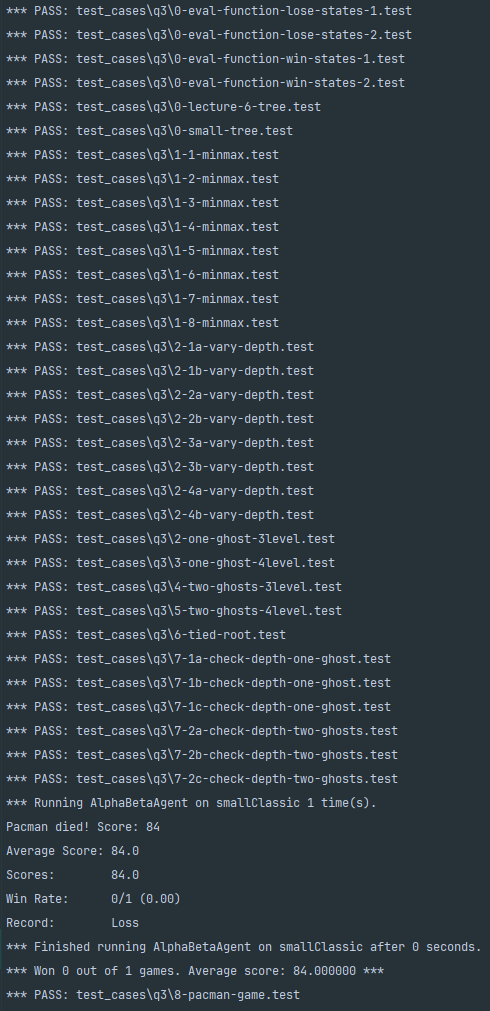
\includegraphics[scale = 0.8]{pic/q3.png}
    \caption{Question3实验结果}\label{q3}
\end{figure}
%
%在算法原理的基础上,结合代码,讲述算法的实现细节、和兴函数、模块输入输出,数据结构定义等内容
%
%
%对试验结果进行详细展示,对每个问题展示测试截图,对于测试用例进行描述说明,对于为通过测试的用例结合自己的算法进行分析,可以结合调试过程进行分析
%
%实验中遇到的问题及解决方案,收获和思考:对算法的理解、优缺点的评价、算法的适用场景
%
